\documentclass[c,8pt,xcolor...,x11names]{beamer}
\usepackage{icclslides}
\usepackage[latin1]{inputenc}
\usepackage[british]{babel}
\usepackage{amssymb}
\usepackage{latexsym}
\usepackage{rotate}
\usepackage{tikz}
\usepackage{verbatim}
\usepackage{colortbl}
\usepackage{booktabs}
\usepackage{ulem}
% \usepackage{arydshln}
\usepackage{pdfpages}
\usepackage{graphicx} 
\usepackage{tikzsymbols}
\usepackage{tikz}
\usepackage{pdfpages}
\usetikzlibrary{positioning}

\tikzstyle{ele} = [circle, text centered, minimum width=1em, minimum height=3ex]

%% Uncomment to activate navigation symbols in the lower right of the pages:
\setbeamertemplate{navigation symbols}{}
\setbeamercovered{transparent}

\renewcommand{\Myauthor}{Martin R\"obke}
\renewcommand{\Mytitle}{Visualizing Dynamic Programming \newline
	On Tree Decompositions}
\usepackage{showexpl} 

\lstloadlanguages{[LaTeX]Tex} 
\lstset{% 
     basicstyle=\ttfamily\small, 
     commentstyle=\itshape\ttfamily\small, 
     showspaces=false, 
     showstringspaces=false, 
     breaklines=true, 
     breakautoindent=true, 
     captionpos=t 
} 

\begin{document} 
\begin{frame}
\customtitle
\begin{list2}
\item {\sc What} is this about?
\item {\sc Who} benefits from visualization?
\end{list2}
\end{frame}

%%%%%%%%%%%%%%%%%
 \section{About me} % taken from Marek Seliger, Matthias Gerdts


 \begin{frame}
  \frametitle{About me}
	
 {\color{blue}Martin R\"obke}
 \medskip

\begin{minipage}{0.6\textwidth}
    \begin{itemize}
    \item[$\bullet$] born in Dresden
    \item[$\bullet$] studying Computer Science Bachelor
    \begin{itemize} \smallskip
    \item[$\bullet$] started studying physics at the TU Dresden
    \item[$\bullet$] did like logic and visualization more, so switched the faculty \quad \Winkey
	\end{itemize}
    \end{itemize}
\end{minipage}\hfill
\begin{minipage}{0.35\textwidth}
	\begin{figure}[H]
			
\includegraphics[height=0.33\textheight]{images/Martincrop.jpg}
	\end{figure}
\end{minipage} 

\bigskip
 {\color{blue}How did I get to work with my supervisor Johannes Fichte?}

\end{frame}

%%%%%%%%%%%%%%%%%%%%%%
\section{Motivation}

\begin{frame}
	\frametitle{Motivation}
	\begin{minipage}{0.7\textwidth}
	\textbf{\color{blue}Previous work:} \medskip
	\begin{itemize}
		\item Boolean formulas are very expressive!
		\pause
		\begin{itemize}
				\item Problem with huge instances
		\end{itemize}
		\pause
		%Using customized algorithms and datastructures and highly parallel hardware
		\item Customized algorithms, data-structures, hardware
	\end{itemize}
	\medskip
	\textbf{\color{blue}Why visualization?}\medskip
	\begin{center}
		{\color{blue}$\rightarrow$ trace and document the customization}
	\end{center}
	\textbf{\color{blue}Outlook:} \medskip
	\begin{itemize}
		\item Improve and streamline the visualization process % API, diff. programs etc. 
		\item Implement debug-output in existing solvers
		%Enable
		\item Even more dynamic possibilities 
	\end{itemize}
	\end{minipage}\hfill
	\begin{minipage}{0.28\textwidth}
		\begin{figure}[H]
			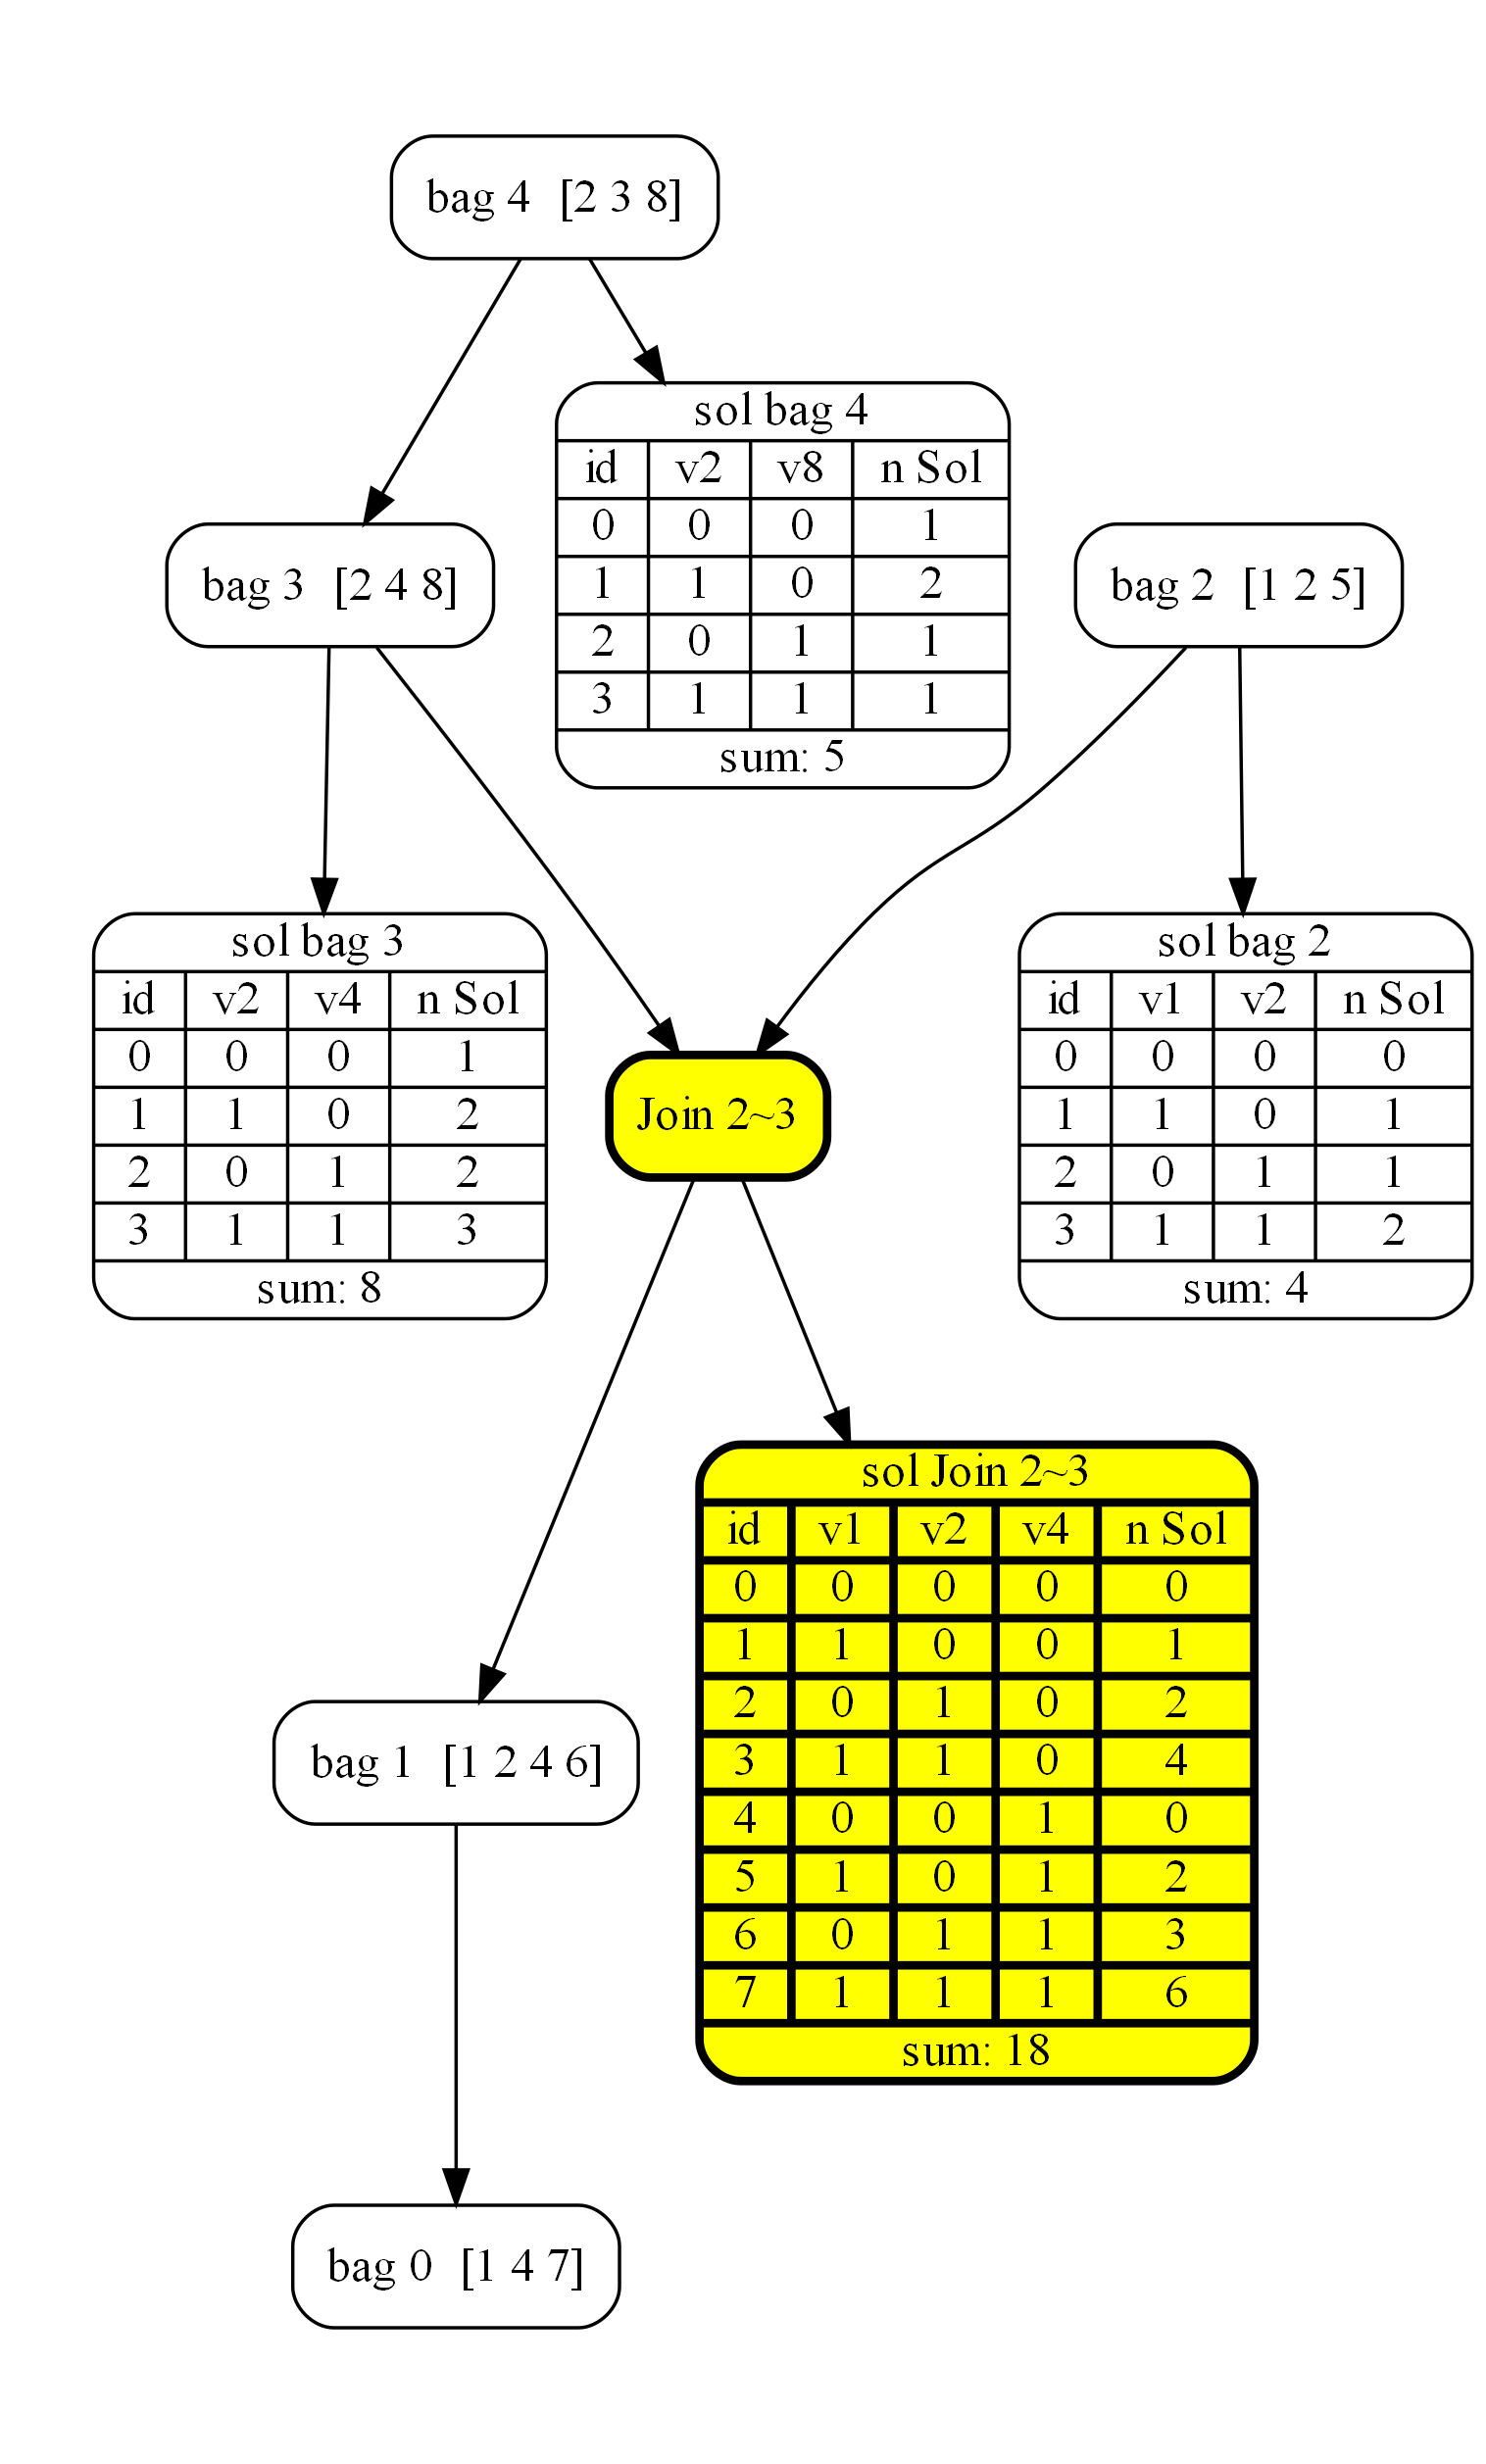
\includegraphics[width=\linewidth]{images/g41DigraphProgress6.png}
			\caption{\label{fig:g416} Example of a \#SAT run with DP}
		\end{figure}
	\end{minipage} 

\end{frame}

%%%%%%%%%%%%%%%%%%%%%
\section{Background}
\subsection{Different extensions of logic}
\begin{frame}
	\frametitle{Background}
	\begin{figure}
		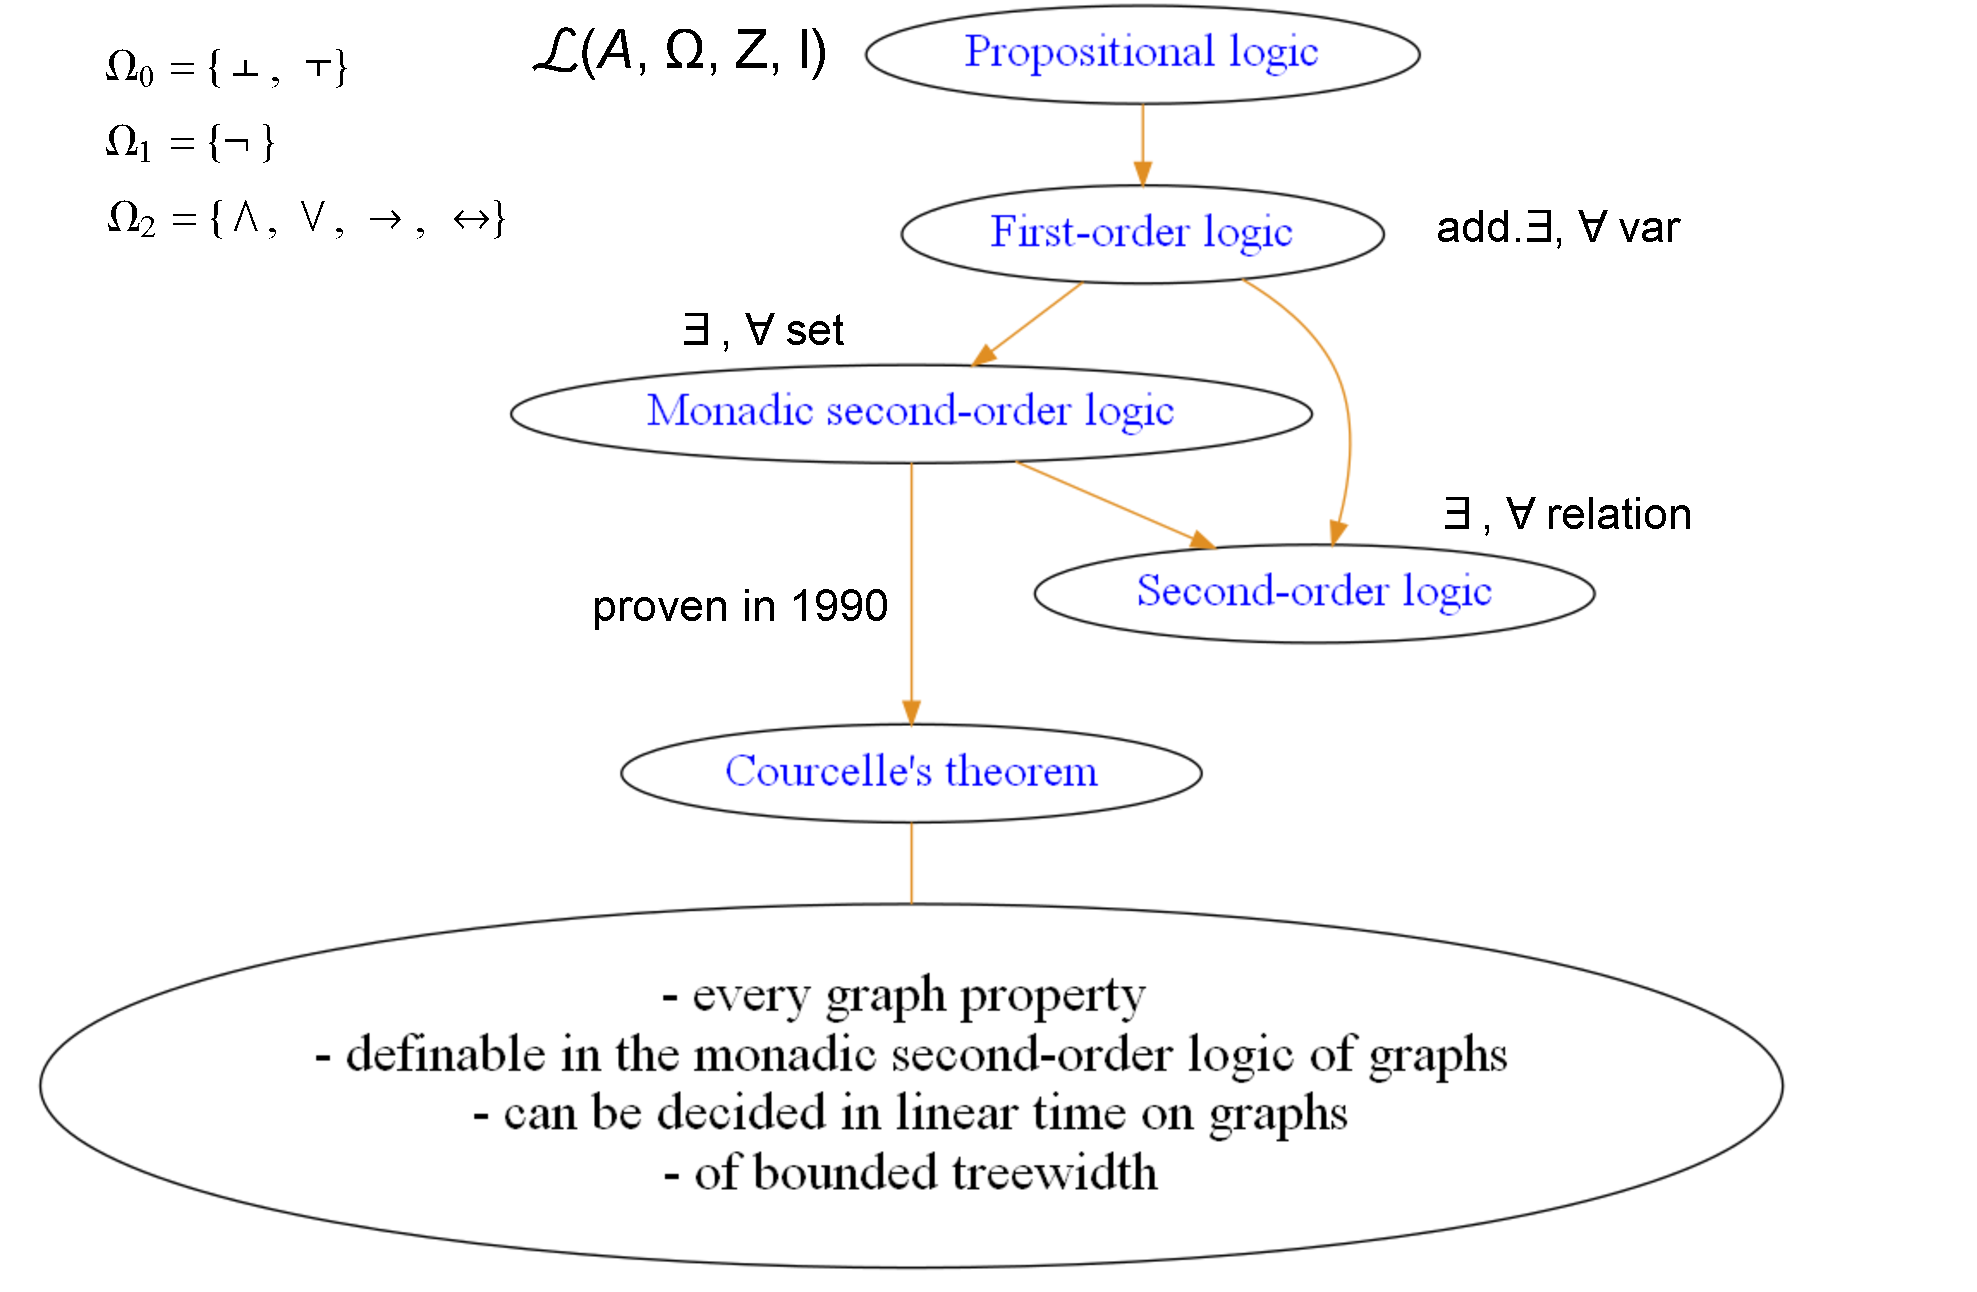
\includegraphics[height=0.9\textheight]{images/DifferentLogicgraph2.pdf}
	\end{figure}
\end{frame}
%%
\subsection{Example Vertex cover}
\begin{frame}
\frametitle[Vertex Cover]{Example: Vertex-Cover problem}

%We take an undirected graph 
%\begin{center}
%	We take an undirected graph	\textbf{G} = (\textbf{V}, \textbf{E})
%\end{center}
%where \textbf{V} is the set of nodes and \textbf{E} the set of edges, each between two elements of \textbf{V}. 
For this graph \textbf{G} we want to compute a \emph{set of vertices} so that from every edge $(u, v)$ there is \emph{at least one} of $u$ or $v$ in that ``cover" of \textbf{G}. \smallskip 

\begin{figure}
	\centering
	\begin{minipage}{0.45\textwidth}
		\centering
		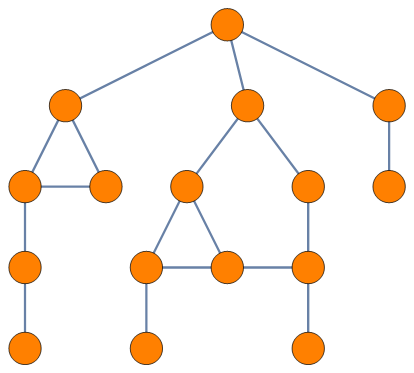
\includegraphics[width=0.6\textwidth]{"images/threeGraph1.png"}
		\caption{Example undirected graph \textbf{G}} 
	\end{minipage}
	\begin{minipage}{0.45\textwidth}
		\centering
		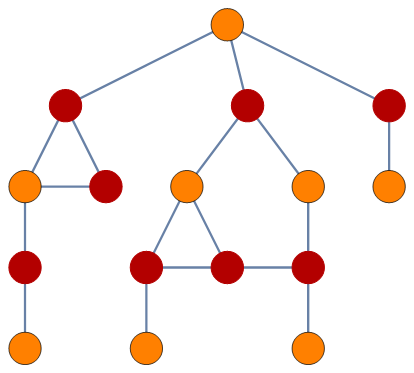
\includegraphics[width=0.6\textwidth]{images/threeGraphOptimal.png} 
		\caption{Minimal VC of \textbf{G}} 
	\end{minipage}
\end{figure}

%The size of the vertex cover is the number of vertices in it.
\hspace*{0.1\textwidth}
\begin{minipage}{0.8\textwidth}
	\begin{center}
		$\exists S: ~\forall x,y \in E: (x\in S \vee  y\in S)$
	\end{center} \medskip
	{\color{blue}Finding the \emph{smallest} of these sets is the optimization version % (how large is the smallest set?) 
		of a NP-complete decision problem. %(is there a vertex cover of size \textit{k}).
	}

\end{minipage}
\end{frame}
%%
\subsection[Courcelle]{Courcelle's theorem}
\begin{frame}
	\frametitle{Courcelle's theorem}
	\pause
	\begin{itemize}
		\item \emph{statement:} \begin{quotation}
			Every graph property definable in MSOL is decidable in linear time on graphs of bounded treewidth. \\
			\hfill {\small Courcelle, Bruno (Bordeaux I University 1990)}
		\end{quotation}
	\medskip \pause
		\item \emph{drawback:} still expensive ($2^{k*tw}$, $2^{2^{\#quant}}$, large constants) \smallskip \pause
		\item \emph{usage:}
		
\end{itemize}
\begin{figure}
	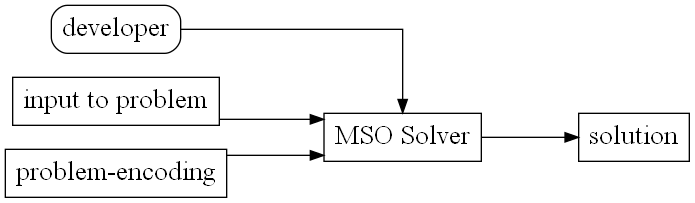
\includegraphics[height=0.2\textheight]{images/UsageCourcelle.gv.png}
	\caption{Implementation of the theorem}
\end{figure}
\end{frame}
%%
\subsection{\#SAT and WMC}
\begin{frame}
	\frametitle{(Weighted) Model-Counting}
% https://en.wikipedia.org/wiki/Sharp-SAT#Intractable_special_cases
	\vspace{.2\textheight}
	{\color{blue} The \#SAT Problem} \\
	Input: A boolean formula \textbf{F} \\
	Question: How many assignments do the occurring variables satisfy in \textbf{F}
	
	\bigskip
	{\color{blue} The Weighted Model Counting Problem}
	\begin{itemize}
		\item $w(lit) \in [0,1], \quad w(� lit) = 1-w(lit)$
		\item $w(assignment) = \prod_{lit} w(lit)$
		\item $WMC(formula) = \sum_{\footnotesize satisfying~~ assignments} w(assignment)$
	\end{itemize}
\end{frame}
\begin{frame}
	\frametitle{Graphs for Boolean Formulas}
	\smallskip
	{\color{blue} Transforming the formula into CNF-form}
	\begin{figure}
		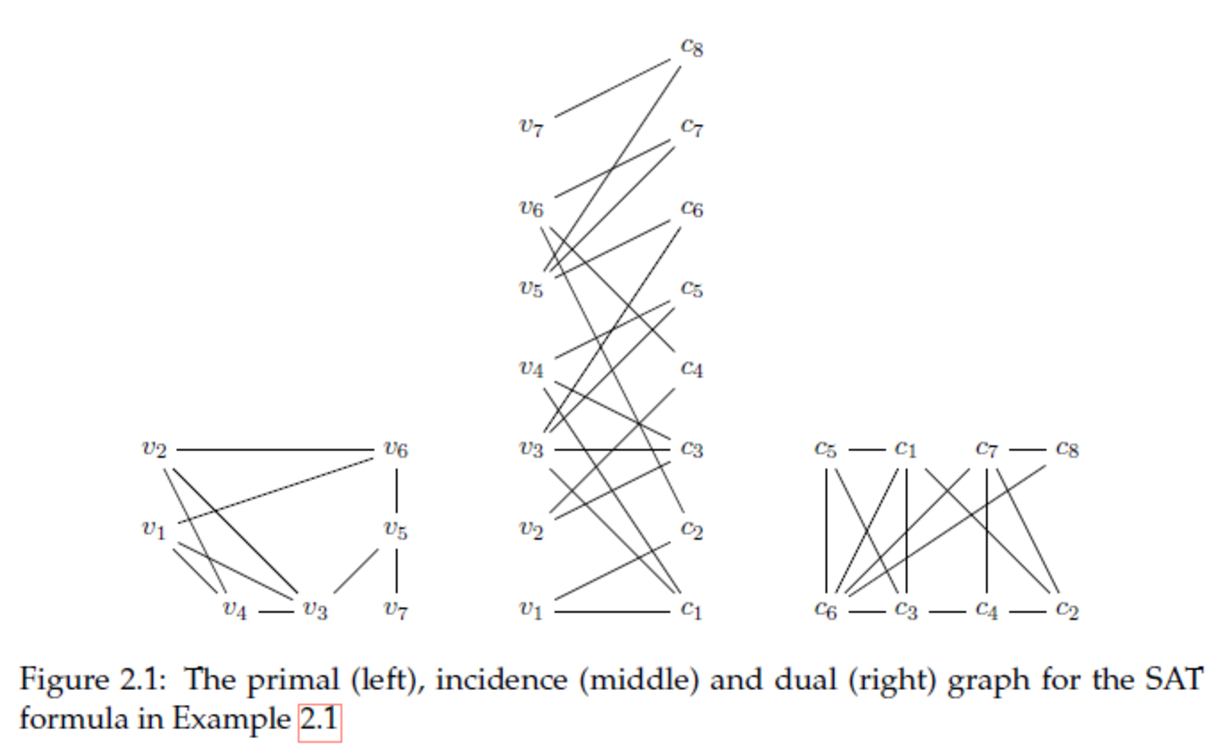
\includegraphics[height=0.7\textheight]{images/DAGraphs.pdf}
	\end{figure}
\end{frame}

%%
\subsection[TD]{Tree decomposition}
\begin{frame}
\frametitle{Tree Decompositions}
{\color{blue}\emph{Parameterized Complexity and its Applications in Practice} \\
From Foundations to Implementations \\
Johannes K. Fichte \\
TU Dresden, Germany \\
Jakarta, Indonesia \\
{Summer 2019 (May 6th - May 16th)}
}

pages 162-174

\emph{Backup: VC tree vs graph - example}
\end{frame}
%{
%	\setbeamercolor{background canvas}{bg=}
%	\includepdf[pages=162-174]{"images/Lecture_pcgp_Summer_2019.pdf"}
%}
%%%%%%%%%%%%%%%%%%%%%%%
\section{implementations}
\subsection{gpusat1}
\begin{frame}
	\frametitle{gpuSAT1}
	graphic / github
	
	\begin{itemize}
	\item OpenCL
	\item Incidence + Primal Graph
	\end{itemize}
\end{frame}
%%
\subsection{gpusat2}
\begin{frame}
	\frametitle{gpuSAT2}
	graphic / github
	
	\begin{itemize}
		\item OpenCL
		\item Only primal graph - simpler solving DP
		\item adapted memory-management
		\item improved precision handling
		\item customized tree decompositions
	\end{itemize}
\end{frame}
%%
\subsection{dpdb}
\begin{frame}
	\frametitle{dpdb}
	graphic / github
	
	\begin{itemize}
		\item using databases for intermediate results
		\item SAT
		\item \#SAT
		\item Vertex Cover
	\end{itemize}
\end{frame}


%%%%%%%%%%%%%%%%%%%%%%%
\section{Visualization}
\subsection{Handcrafted}
\begin{frame}
	\frametitle{TODO - DA}
	\begin{figure}
		\centering
		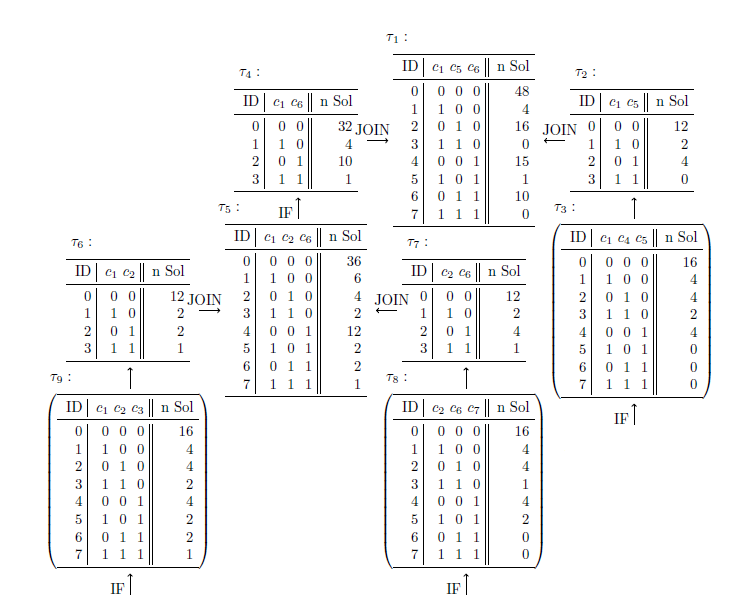
\includegraphics[width=0.7\linewidth]{images/DualDA43}
		\caption{Handcrafted \#SAT example-run from Markus Zisser}
		\label{fig:dualda43}
	\end{figure}

\end{frame}
\begin{frame}
	\frametitle{TODO - presentation\_gpusat}
	
\end{frame}

%%%%%%%%%%%%%%%%%%%%%%%
\section{Further Visualization}
\begin{frame}
\frametitle{Creating Visualization for:}
\emph{Improving}
\begin{itemize}
	\item documentation 
	\item debugging complex ds and parallel sync
	\item hotspots
\end{itemize}
\emph{Generalizing the underlying graph structure}
\end{frame}

%%%%%%%%%%%%%%%%%%%%%%%
\section{Outlook}
\begin{frame}
	\frametitle{Outlook}
	\begin{itemize}
		\item customizable output and interactive visualization
		\item ref. impl. in CUDA of gpuSAT2 
	\end{itemize}
\end{frame}

%%%%%%%%%%%%%%%%%%%%%%%
\section{Further Information}

\begin{frame}
 \frametitle{Further Information}
\begin{itemize}
\item
\end{itemize}

\end{frame}

%%%%%%%%%%%%%%%%%%%%%%%
\section{References}

\begin{frame}
\frametitle{References}

\begin{itemize}
\item
\end{itemize}

\end{frame}

\bgroup
\setbeamercolor{background canvas}{bg=black}
\begin{frame}[plain]{}
\end{frame}
\egroup

\end{document}
